\section{Rearrangement and repair}\label{sec:rearrange}

This chapter turns the single moves of Sec.~\ref{sec:transport} into a full rearrangement cycle, counts its passes, time and moves per atom, and asks what limits the probability of a defect-free block. A 16-chip stack with row select assembles a defect-free $32\times32$ block from a $50\times45$ array loaded at 50\% in 17.2~ms on average over 40 loadings (worst 23.0~ms), with 5.8 balancing and 2 compaction passes. Every loading succeeded before losses were applied. The average atom in the block moves 1.12 times and none moves more than twice, so with the slow handoff steps the finished block is no more than about 0.6~\textmu K hotter than at the start. One round of imaging and repair then takes 10 to 13~ms. The outcome is set by losses, not by the scheduler: by the loss per move, the loss per image and the vacuum lifetime. The photonic chip contributes 1.1 moves per atom and 17~ms per cycle; reaching a 99\% defect-free block requires each loss term near $10^{-5}$, which is a property of the platform.

\subsection{Hardware rules and scheduler}\label{sec:rearrange-scheduler}

The hardware sets three rules: (i) a stack addresses 16 consecutive rows at a time; (ii) every tweezer of the stack shares the $y$ motion (into the lane 2~\textmu m off the row, optionally along mid-column lanes over $j$ rows, and back), while each tweezer moves independently in $x$; (iii) tweezers in one row keep their order and so stay at least 4~\textmu m apart. The scheduler works in two stages. In vertical balancing, each pass chooses a stack position $k$ and a common row shift $j$ that move the most surplus atoms into target rows lacking atoms. Arriving atoms go straight to empty target columns where possible, and atoms that arrive in a pass are not picked again in the same pass. In horizontal compaction, one pass per group of 16 target rows matches each row's atoms in order to the target columns and pushes the extras just outside the block.

A pass takes two ramps, two lane steps, the $x$ moves (minimum jerk, 400~\textmu s per 40~\textmu m, scaled as $\sqrt{d}$ with the distance $d$, at least 200~\textmu s), the $y$ travel for $j$ rows, and 0.3~ms of scanner settling (our choice). Of the 2.2~ms of a typical pass, ramps, lane steps and settling make up 1.3~ms. The schedule is greedy and not optimal: a planner that combines balancing and compaction, or shares passes between stack positions, would need fewer passes. Section~\ref{sec:rearrange-modes} shows how much better pass selection gains.

\subsection{Cycle time and moves per atom}\label{sec:rearrange-cycle}

Table~\ref{tab:rearrange-cycle} lists the cycle for several targets and loadings, and Fig.~\ref{fig:rearrange-cycle} shows the mean cycle time. A larger target from the same $50\times45$ array costs more balancing passes ($36\times36$ at 60\% needs 8.3 + 3 and 25.1~ms on average), while a higher loading saves them (32$\times$32 at 60\%: 14.8~ms). A second stack, combined with the first to address 32 rows, does not change the number of balancing passes but saves one compaction pass (15.5 against 17.2~ms for the $32\times32$ block at 50\%). The number of moves per atom stays near 1.1 in every case: about 22\% of the atoms in the $32\times32$ block at 50\% loading move twice, the rest once or not at all.

\begin{table}[htbp]\centering\small
\caption{One rearrangement cycle from a $50\times45$ array, mean over 40 random loadings, base timing (100~\textmu s ramps, 400~\textmu s lane steps, 0.3~ms settling); passes are vertical (V, balancing) plus horizontal (H, compaction). Defects are expected numbers in the block, from the assumed loss per move (moves) and from vacuum loss during the cycle at lifetimes of 30 and 300~s (vacuum). Simulated; loss rates assumed.}
\label{tab:rearrange-cycle}
\setlength{\tabcolsep}{3.5pt}
\begin{tabular}{lllllll}
\toprule
target & rows & passes & cycle (ms) & moves/atom & defects, moves & defects, vacuum \\
(loading) & & V + H & mean / max & mean / max & $10^{-3}$ / $10^{-4}$ & 30 / 300~s \\
\midrule
$30\times30$ (50\%) & 16 & 4.3 + 2 & 13.3 / 17.1 & 1.11 / 2 & 1.00 / 0.10 & 0.40 / 0.04 \\
$32\times32$ (50\%) & 16 & 5.8 + 2 & 17.2 / 23.0 & 1.12 / 2 & 1.15 / 0.12 & 0.59 / 0.06 \\
$32\times32$ (60\%) & 16 & 5.0 + 2 & 14.8 / 17.1 & 1.03 / 2 & 1.06 / 0.11 & 0.50 / 0.05 \\
$36\times36$ (60\%) & 16 & 8.3 + 3 & 25.1 / 35.6 & 1.07 / 2 & 1.38 / 0.14 & 1.08 / 0.11 \\
$32\times32$ (50\%) & 32 & 5.8 + 1 & 15.5 / 21.3 & 1.12 / 2 & 1.15 / 0.12 & 0.53 / 0.05 \\
\bottomrule
\end{tabular}
\end{table}

\begin{figure}[htbp]\centering
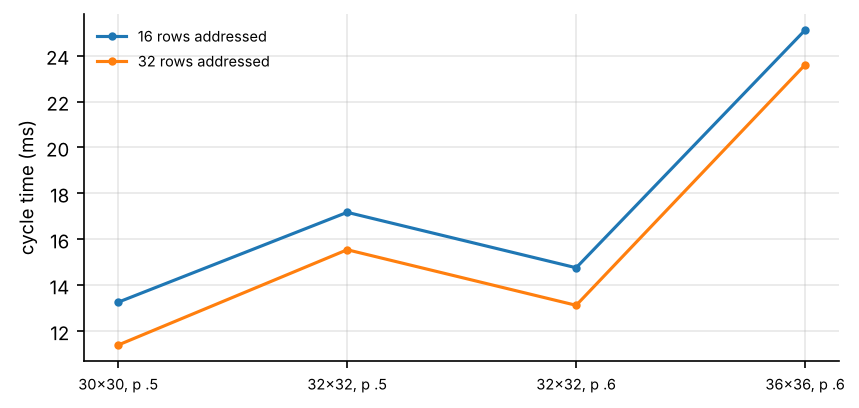
\includegraphics[width=0.8\linewidth]{m20_rearrange.png}
\caption{Mean cycle time of one rearrangement cycle (greedy scheduler, 40 random loadings of a $50\times45$ array at 4~\textmu m pitch) for four target blocks and loading probabilities $p$, with one 16-chip stack (16 rows addressed) and two combined stacks (32 rows addressed). Timing: 100~\textmu s ramps, 400~\textmu s lane steps, minimum-jerk $x$ moves of 400~\textmu s per 40~\textmu m scaled as $\sqrt{d}$ (at least 200~\textmu s), 0.3~ms scanner settling per pass. The second stack saves one compaction pass in each case.}
\label{fig:rearrange-cycle}
\end{figure}

The cycle time depends mainly on the fixed costs of a pass (Table~\ref{tab:rearrange-timing}). The low-heating steps of Sec.~\ref{sec:transport-timing} raise it from 17.2 to 18.8~ms. Shortening the lane steps to 100~\textmu s gives 12.5~ms, and making everything fast gives 8.2~ms, while slower scanner settling (1~ms) gives 22.7~ms. Because vacuum loss grows with cycle time, the all-fast setting halves it (0.28 defects at 30~s). It costs heating: about 10~\textmu K per move at a moving depth of 0.3~mK, or 1.2~\textmu K at 0.5~mK. Thus two regimes remain: slow and cold at 0.3~mK, with low power, or fast at 0.5~mK. With the slow steps (0.29~\textmu K per move, lateral handoff plus $x$ move) the block gains 0.33~\textmu K on average and 0.58~\textmu K for an atom moved twice; with fast steps at 0.5~mK the corresponding figures are 1.36 and 2.42~\textmu K.

\begin{table}[htbp]\centering\small
\caption{Sensitivity of the cycle time to the step timing ($32\times32$ block, 50\% loading, one stack, mean of 40 loadings; simulated).}
\label{tab:rearrange-timing}
\begin{tabular}{ll}
\toprule
timing & cycle time \\
\midrule
base (ramps 100~\textmu s, lane steps 400~\textmu s) & 17.2~ms \\
low heating (ramps 200~\textmu s, lane steps 400~\textmu s) & 18.8~ms \\
fast lane steps (100~\textmu s) & 12.5~ms \\
all fast (ramps 50~\textmu s, lane steps 100~\textmu s, $x$ 200~\textmu s per 40~\textmu m) & 8.2~ms \\
scanner settling 1~ms instead of 0.3~ms & 22.7~ms \\
\bottomrule
\end{tabular}
\end{table}

\subsection{Pass selection and the pass floor}\label{sec:rearrange-modes}

We compared three ways of selecting the balancing passes on 40 loadings ($32\times32$, 50\%, one stack): greedy (most atoms per pass), rate (most atoms per unit pass time) and lookahead (best two-pass sequence among the 8 best first passes). They need 8.05, 8.05 and 7.98 passes in all, with mean cycle times of 17.8, 17.6 and 17.6~ms (maxima 23.1, 22.8 and 22.9~ms). The three modes agree to within 1\%. This is because the balancing stage has a geometric floor of about four passes. In one pass the 16-row window can hold at most 9 non-target rows above or below the 32-row target band, so it can feed at most 9 target rows; feeding all 32 therefore takes at least four passes, plus two compaction passes. The greedy schedule (5.8 + 2) is within about 30\% of that floor. Further gains would come from shorter passes, not from fewer.

\subsection{Stochastic losses and defects}\label{sec:rearrange-loss}

The scheduler fills every loading; defects come from losses. The loss per move is not computed by the transport simulations, which bound it below about $10^{-3}$ (0 of 3,000 atoms lost); we take $10^{-3}$ and $10^{-4}$, the latter an assumption. Vacuum lifetimes of 30 and 300~s are also assumed. At $10^{-3}$ per move the $32\times32$ cycle leaves 1.15 defects on average and at $10^{-4}$ 0.12; vacuum loss during the 17~ms adds 0.59 defects at 30~s and 0.06 at 300~s (Table~\ref{tab:rearrange-cycle}). The probability that the block is defect-free after one cycle is 0.84 at $10^{-4}$ per move and 300~s. Reaching 0.99 in one cycle would need about $5\times10^{-6}$ loss per move and a vacuum lifetime above about one hour. A repair round after imaging is the realistic route.

\subsection{Image-and-repair rounds}\label{sec:rearrange-repair}

After the cycle, the array is imaged (10~ms, our choice) and each hole in the block is filled directly by one reservoir atom, moved through the lanes from the nearest rows under the same pass rules. This takes 0.1 to 1.3 repair passes, so a round lasts 10 to 13~ms. The repair works, but it cannot go below a floor set by the image itself: atoms lost because of the image are not seen by it, and every atom is exposed to vacuum loss for the duration of the round. The expected number of defects after a round is
\begin{equation}
  n_\mathrm{d} \approx N\left(\epsilon_\mathrm{img} + \frac{t_\mathrm{round}}{\tau}\right) + p_\mathrm{move}\, n_\mathrm{rep}.
  \label{eq:rearrange-floor}
\end{equation}
Here, $N=1024$ is the number of sites in the block, $\epsilon_\mathrm{img}$ the loss per image, $t_\mathrm{round}$ the duration of the round, $\tau$ the vacuum lifetime, $p_\mathrm{move}$ the loss per move and $n_\mathrm{rep}$ the number of repair moves. For $\epsilon_\mathrm{img}=10^{-4}$ and $\tau=300$~s this gives about 0.14 defects, and a second round does not lower it (Table~\ref{tab:rearrange-repair}).

\begin{table}[htbp]\centering\small
\caption{Probability of a defect-free $32\times32$ block after the cycle and after one and two image-and-repair rounds, and expected defects after one round (simulated, 40 loadings $\times$ 25 loss draws per row; all loss rates and lifetimes assumed).}
\label{tab:rearrange-repair}
\setlength{\tabcolsep}{3.5pt}
\begin{tabular}{lllll}
\toprule
loss per move & lifetime & loss per image & P(defect-free): cycle / 1 / 2 rounds & defects after 1 repair \\
\midrule
$10^{-3}$ & 300~s & $10^{-4}$ & 0.27 / 0.87 / 0.87 & 0.14 \\
$10^{-4}$ & 300~s & $10^{-4}$ & 0.84 / 0.87 / 0.87 & 0.14 \\
$10^{-3}$ & 300~s & $10^{-3}$ & 0.27 / 0.35 / 0.33 & 1.04 \\
$10^{-4}$ & 300~s & $10^{-3}$ & 0.84 / 0.35 / 0.33 & 1.03 \\
$10^{-3}$ & 30~s & $10^{-4}$ & 0.14 / 0.59 / 0.62 & 0.53 \\
$10^{-4}$ & 30~s & $10^{-4}$ & 0.48 / 0.62 / 0.63 & 0.48 \\
\bottomrule
\end{tabular}
\end{table}

As can be seen from Table~\ref{tab:rearrange-repair}, a repair round brings poor transport ($10^{-3}$ per move) up to the same 0.87 as good transport, provided the image is gentle. Once the loss per move is about $10^{-4}$ or less, the probability of a defect-free block is set by the imaging loss and the vacuum lifetime, not by the transport. With good transport and an imaging loss of $10^{-3}$, a repair round makes things worse: 0.84 becomes 0.35, because the image costs about one atom of the block. Imaging should then be skipped, or used only to post-select. For a 99\% defect-free block each term of Eq.~\eqref{eq:rearrange-floor} must be near $10^{-5}$: the loss per move, the loss per image, and $t_\mathrm{round}/\tau$. The continuous version of this balance, with periodic imaging and refilling of much larger arrays, is the subject of Sec.~\ref{sec:megascale}.

\subsection{Limits}\label{sec:rearrange-limits}

The scheduler is greedy and not optimised across stack positions. The loss per move is bounded by the transport simulations but not computed, and the values used here, like the imaging time, imaging loss and vacuum lifetimes, are assumptions. Detection is taken as perfect apart from the imaging-induced loss, with no false positives or negatives. The repair model moves one reservoir atom per hole. Photon scattering by the trapping light (estimated at a few photons per second at 0.3 to 0.5~mK) is not included, and neither is the possibility that an atom heated by its moves is lost during later moves. The heating per move comes from the one-dimensional quantum check and the three-dimensional classical runs of Sec.~\ref{sec:transport-timing}, with the axial focus offset held to $\pm0.5$~\textmu m (Sec.~\ref{sec:transport-tol}).
